\chapter{Технологический раздел}

\section{Средства разработки}

Для реализации поддерживающего спроектированный протокол ПО был выбран язык С.
В качестве средства сборки используется средство сборки CMake \cite{cmake}.

Для работы с медиа данными используется библиотека с открытым исходным кодом \texttt{ffmpeg} \cite{ffmpeg}.

Шифрование сообщений осуществляется с использованием библиотеки \texttt{OpenSSL}.

Для автотестов используется фреймворк \texttt{GoogleTest} \cite{gtest}.

\section{Листинги процедуры приглашения}

\noindent
Листинг 3.1 --- Процедура приглашения со стороны приглашающего

{\fontsize{11pt}{2pt}\selectfont
\begin{verbatim}
static enum SError do_handshake_client(struct SConnection *con,
    struct SMessage *msg, struct SMsgInviteAccept **acceptMsg) {
  enum SError err = sconn_send(con, msg);
  if (err != SELECON_OK)
    return err;
  err = sconn_recv(con, &msg);
  if (err != SELECON_OK)
    message_free(&msg);
  else if (msg->type == SMSG_INVITE_ACCEPT)
    *acceptMsg = (struct SMsgInviteAccept *)msg;
  else {
    message_free(&msg);
    err = SELECON_INVITE_REJECTED;
  }
  return err;
}
\end{verbatim}}

\noindent
Листинг 3.2 --- Процедура приглашения со стороны приглашаемого

{\fontsize{11pt}{9pt}\selectfont
\begin{verbatim}
static enum SError do_handshake_srv(struct SParticipant *self,
    struct SEndpoint *listen_ep, struct SConnection *con,
    struct SMsgInvite **invite, invite_handler_fn_t handler) {
  struct SMessage *msg = NULL;
  enum SError err      = sconn_recv(con, &msg);
  if (err != SELECON_OK || msg->type != SMSG_INVITE)
    goto cleanup;
  bool accepted = handler((struct SMsgInvite *)msg);
  if (!accepted) {
    msg->size = sizeof(struct SMessage);
    msg->type = SMSG_INVITE_REJECT;
    err       = sconn_send(con, msg);
    goto cleanup;
  }
  *invite = (struct SMsgInvite *)msg;
  msg     = message_invite_accept_alloc(self->id, self->name, listen_ep);
  err     = sconn_send(con, msg);
cleanup:
  message_free(&msg);
  return err;
}
\end{verbatim}}

\noindent
Листинг 3.3 --- Воркер, обрабатывающий входящие приглашения в конференции

{\fontsize{11pt}{9pt}\selectfont
\begin{verbatim}
static void *invite_worker(void *arg) {
  struct SContext *ctx           = arg;
  struct SConnection *listen_con = NULL;
  enum SError err                = sconn_listen(&listen_con, &ctx->listen_ep);
  while (ctx->initialized && (err == SELECON_OK || err == SELECON_CON_TIMEOUT)) {
    struct SConnection *con = NULL;
    err = sconn_accept_secure(listen_con, &con, SELECON_DEFAULT_SECURE_TIMEOUT);
    if (err == SELECON_OK) {
      struct SMsgInvite *invite = NULL;
      err = do_handshake_srv(&ctx->self, &ctx->listen_ep, con, &invite,
              ctx->invite_handler);
      if (err == SELECON_OK && invite != NULL)
        err = handle_invite(ctx, con, invite);
      if (err != SELECON_OK || invite == NULL)
        sconn_disconnect(&con);
      message_free((struct SMessage **)&invite);
    }
  }
  sconn_disconnect(&listen_con);
  return NULL;
}
\end{verbatim}}

Листинг 3.4 --- Процедура приглашения участника в конференцию

{\fontsize{11pt}{9pt}\selectfont
\begin{verbatim}
static enum SError invite_connected(struct SContext *context,
    struct SConnection *con, part_id_t *out_part_id) {
  struct SMessage *inviteMsg = message_invite_alloc(
      context->conf_id, context->conf_start_ts, context->self.id, context->self.name);
  struct SMsgInviteAccept *acceptMsg = NULL;
  enum SError err                    = do_handshake_client(con, inviteMsg, &acceptMsg);
  if (err != SELECON_OK || acceptMsg == NULL)
    return err;
  // send other participants info about invitee
  struct SMsgPartPresence *msg = message_part_presence_alloc();
  msg->part_id                 = acceptMsg->part_id;
  msg->ep                      = acceptMsg->ep;
  msg->part_role               = SROLE_CLIENT;
  msg->state                   = PART_JOIN;
  pthread_rwlock_wrlock(&context->part_rwlock);
  for (size_t i = 0; i < context->nb_participants - 1; ++i)
    sconn_send(context->participants[i].connection, (struct SMessage *)msg);
  add_participant(context, acceptMsg->id, acceptMsg->name, con);
  if (context->nb_participants == 2 && !context->conf_thread_working) {
    pthread_create(&context->conf_thread, NULL, conf_worker, context);
    pthread_setname_np(context->conf_thread, "conf");
  }
  pthread_rwlock_unlock(&context->part_rwlock);
  *out_part_id = acceptMsg->part_id;
  message_free((struct SMessage **)&msg);
  message_free((struct SMessage **)&acceptMsg);
  return SELECON_OK;
}
\end{verbatim}}

Листинг 3.5 --- Процедура повторного подключения к конференции

{\fontsize{11pt}{9pt}\selectfont
\begin{verbatim}
enum SError selecon_reenter(struct SContext *context) {
  struct SMsgReenter *msg = message_reenter_alloc(context->conf_id, context->self.id);
  enum SError err         = SELECON_OK;
  pthread_rwlock_rdlock(&context->part_rwlock);
  for (size_t i = 0; i < context->nb_participants - 1; ++i) {
    struct SConnection *con = NULL;
    err = sconn_connect_secure(&con, &context->participants[i].listen_ep);
    if (err != SELECON_OK) {
      sconn_disconnect(&con); break;
    }
    err = sconn_send(con, (struct SMessage *)msg);
    if (err != SELECON_OK) {
      sconn_disconnect(&con); break;
    }
    err = sconn_recv(con, (struct SMessage **)&msg);
    if (err != SELECON_OK) {
      sconn_disconnect(&con); break;
    }
    // restore participant state and streams
    if (!spart_hangup_validate(&context->participants[i], con))
      err = SELECON_CON_TIMEOUT;
    else {
      sstream_id_t audio_stream = NULL;
      sstream_id_t video_stream = NULL;
      err = scont_alloc_stream(&context->streams, context->participants[i].id,
        context->conf_start_ts, SSTREAM_AUDIO, SSTREAM_INPUT, &audio_stream);
      assert(err == SELECON_OK);
      err = scont_alloc_stream(&context->streams, context->participants[i].id,
        context->conf_start_ts, SSTREAM_VIDEO, SSTREAM_INPUT, &video_stream);
      assert(err == SELECON_OK);
    }
  }
  pthread_rwlock_unlock(&context->part_rwlock);
  message_free((struct SMessage **)&msg);
  if (err != SELECON_OK) {
    // give up reentering - reset context state to new conference
    selecon_leave_conference(context);
  }
  return err;
}
\end{verbatim}}

Листинг 3.6 --- Функции подключения с использованием шифрования

{\fontsize{11pt}{9pt}\selectfont
\begin{verbatim}
static atomic_int ssl_usage_counter = 0;
static void ssl_init(void) {
	if (atomic_fetch_add(&ssl_usage_counter, 1) == 0) {
		SSL_load_error_strings();
		OpenSSL_add_all_algorithms();
	}
}
static void ssl_destroy(void) {
	if (atomic_fetch_add(&ssl_usage_counter, -1) == 1) {
		ERR_free_strings();
		EVP_cleanup();
	}
}
static SSL_CTX *ssl_new_server_ctx(void) {
	const char *cert = cert_get_cert_path();
	const char *key  = cert_get_key_path();
	if (cert == NULL || key == NULL)
		return NULL;
	SSL_CTX *ctx = SSL_CTX_new(SSLv23_server_method());
	if (SSL_CTX_use_certificate_file(ctx, cert, SSL_FILETYPE_PEM) > 0) {
		if (SSL_CTX_use_PrivateKey_file(ctx, key, SSL_FILETYPE_PEM) > 0) {
			return ctx;
		}
	}
	SSL_CTX_free(ctx);
	return NULL;
}
static SSL_CTX *ssl_new_client_ctx(void) {
	SSL_CTX *ctx = SSL_CTX_new(SSLv23_client_method());
	SSL_CTX_set_mode(ctx, SSL_MODE_AUTO_RETRY);
	SSL_CTX_set_verify(ctx, SSL_VERIFY_NONE, NULL);
	return ctx;
}

enum SError sconn_accept_secure(struct SConnection *con,
    struct SConnection **out_con, int timeout_ms) {
  enum SError err = sconn_accept(con, out_con, timeout_ms);
  if (err != SELECON_OK)
    return err;
  ssl_init();
  if (((*out_con)->ssl_ctx = ssl_new_server_ctx()) != NULL) {
    (*out_con)->ssl = SSL_new((*out_con)->ssl_ctx);
    SSL_set_fd((*out_con)->ssl, (*out_con)->fd);
    if (SSL_accept((*out_con)->ssl) > 0)
      return SELECON_OK;
  }
  ERR_print_errors_fp(stderr);
  sconn_disconnect(out_con);
  return SELECON_SSL_ERROR;
}

enum SError sconn_connect_secure(struct SConnection **con, struct SEndpoint *ep) {
	enum SError err = sconn_connect(con, ep);
	if (err != SELECON_OK)
		return err;
	ssl_init();
	if (((*con)->ssl_ctx = ssl_new_client_ctx()) != NULL) {
		(*con)->ssl = SSL_new((*con)->ssl_ctx);
		SSL_set_fd((*con)->ssl, (*con)->fd);
		if (SSL_connect((*con)->ssl) > 0)
			return SELECON_OK;
	}
	ERR_print_errors_fp(stderr);
	sconn_disconnect(con);
	return SELECON_SSL_ERROR;
}
\end{verbatim}}

Листинг 3.7 --- Функции работы с медиа потоками

{\fontsize{11pt}{9pt}\selectfont
\begin{verbatim}
static void stream_input_worker(struct SStream *stream) {
  int64_t pts           = 0;
  struct AVFrame *frame = av_frame_alloc();
  enum AVMediaType mtype = stream->type == SSTREAM_AUDIO
    ? AVMEDIA_TYPE_AUDIO : AVMEDIA_TYPE_VIDEO;
  struct AVPacket *packet = NULL;
  do {
    av_packet_free(&packet);
    packet  = pop_packet(stream);
    int ret = avcodec_send_packet(stream->codec_ctx, packet);
    if (ret < 0) {
      av_frame_free(&frame); break;
    }
    while (ret == 0) {
      ret = avcodec_receive_frame(stream->codec_ctx, frame);
      if (ret < 0) break;
      frame->time_base = stream->codec_ctx->time_base;
      if (mtype == AVMEDIA_TYPE_AUDIO) {
        frame->pts = frame->pkt_dts = pts;
        pts += frame->nb_samples;
      }
      stream->media_handler(stream->media_user_data, stream->part_id, mtype, frame);
      av_frame_unref(frame);
    }
    if (ret != AVERROR(EAGAIN) && ret != AVERROR_EOF)
      perror("avcodec_receive_packet");
  } while (packet != NULL);
  av_frame_free(&frame);
}

static void stream_output_worker(struct SStream *stream) {
	struct AVPacket *packet = av_packet_alloc();
	timestamp_t ts          = 0;
	while (true) {
		struct AVFrame *frame = pop_frame(stream);
		if (frame == NULL) {  // close requested
			av_packet_free(&packet); break;
		}
		int ret = mfgraph_send(&stream->filter_graph, frame);
		if (ret < 0) {
			fprintf(stderr, "mgraph_send: err = %d\n", ret);
			continue;
		}
		while ((ret = mfgraph_receive(&stream->filter_graph, frame)) >= 0) {
			if (frame != NULL) {
				assert(stream->codec_ctx->time_base.num != 0);
				frame->time_base = stream->codec_ctx->time_base;
				frame->pts = av_rescale_q(get_curr_timestamp()
          - stream->start_ts, av_make_q(1, 1000000000), frame->time_base);
				frame->pkt_dts = frame->pts;
			}
			timestamp_t expected_delta = 0; // reduce processing rate
			if (frame->nb_samples > 0)
				expected_delta = av_rescale(frame->nb_samples, 1000000000LL,
          frame->sample_rate);
			else expected_delta = 1000000000LL / SELECON_DEFAULT_VIDEO_FPS;
			reduce_fps(expected_delta, &ts);
			int ret = avcodec_send_frame(stream->codec_ctx, frame);
			if (ret < 0) {
				av_packet_free(&packet);
				av_frame_free(&frame);
				return;
			}
			while (ret == 0) {
				ret = avcodec_receive_packet(stream->codec_ctx, packet);
				if (ret == AVERROR(EAGAIN)) break;
				else if (ret < 0) break;
				stream->packet_handler(stream->packet_user_data, stream, packet);
				av_packet_unref(packet);
			}
			if (ret != AVERROR(EAGAIN) && ret != AVERROR_EOF)
				perror("avcodec_receive_packet");
		}
		if (ret != AVERROR(EAGAIN))
			fprintf(stderr, "mfgraph_receive: err = %d\n", ret);
		av_frame_free(&frame);
	}
}
\end{verbatim}}

\clearpage

\section{Сборка и запуск}

Сборка основного проекта осуществляется с использованием утилиты cmake:

{\fontsize{11pt}{9pt}\selectfont
\begin{verbatim}
  mkdir build
  cd build
  cmake ..
  make цель
\end{verbatim}}
где \textit{<<цель>>} может быть \texttt{selecon\_cli} для сборки консольной утилиты, либо \texttt{unittests} для сборки тестов.

Консольная утилита имеет следующие параметры запуска:

{\fontsize{11pt}{9pt}\selectfont
\begin{verbatim}
$ ./selecon_cli --help
./selecon_cli [OPTIONS]

  example demo application for selecon protocol

OPTIONS:
  -h|--help              show this message
  -l|--listen-on address current participant address (default 0.0.0.0:11235)
  -u|--user username     set user name
  --version              print version and exit
  --stub filename        stream given media file in a loop

DESCRIPTION:
  Address can be IPv4/IPv6 (eg: 192.168.100.1:11235) or socket file path
  in format file://<os-path-to-socket>.
\end{verbatim}}

Список команд, поддерживаемых утилитой:

{\fontsize{11pt}{9pt}\selectfont
\begin{verbatim}
$ ./selecon_cli
> help
list of available commands:
  dev     manage IO devices
  dump    print info about current selecon context state
  exit    end active conference and close cli tool
  help    show this message
  invite  send invitation for joining active conference to other client
  leave   exit conference without exiting cli tool
  quit    same as exit
  say     send text message to conference chat
  sleep   sleep
  stub    set stub media file for playing in conference
\end{verbatim}}

В качестве видео заглушки можно использовать видео файлы в формате MP4.

\clearpage

\section{Тестирование ПО}

Ниже приведен список автотестов, разработанных для проверки реализованного протокола. 

\begin{itemize}[label=---]
  \item Подключение второго участника к конференции, второй участник отклонил приглашение.
  \item Подключение второго участника к конференции, второй участник принял приглашение.
  \item Отправка аудио данных от одного участника другому.
  \item Отправка видео данных от одного участника другому.
  \item Подключение четырех участников к конференции.
  \item Отправка аудио данных от одного участника к другим трем.
  \item Отправка видео данных от одного участника к другим трем.
\end{itemize}

\section{Трассировка пакетов}

На рисунке \ref{img:trace-conf-2} представлен сниф пакетов с использованием программы wireshark \cite{wireshark} во время инициализации конференции с двумя участниками.
На рисунке \ref{img:trace-conf-2-tls} представлен сниф того же сценария, но с использованием TLS протокола.

\begin{figure}[h!]
  \centering
  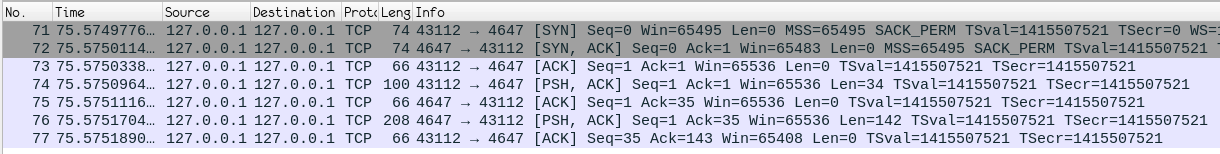
\includegraphics[width=\linewidth]{inc/img/trace-conf-2.png}
  \caption{Сниф wireshark соединения двух участников без использования TLS}
  \label{img:trace-conf-2}
\end{figure}

\begin{figure}[h!]
  \centering
  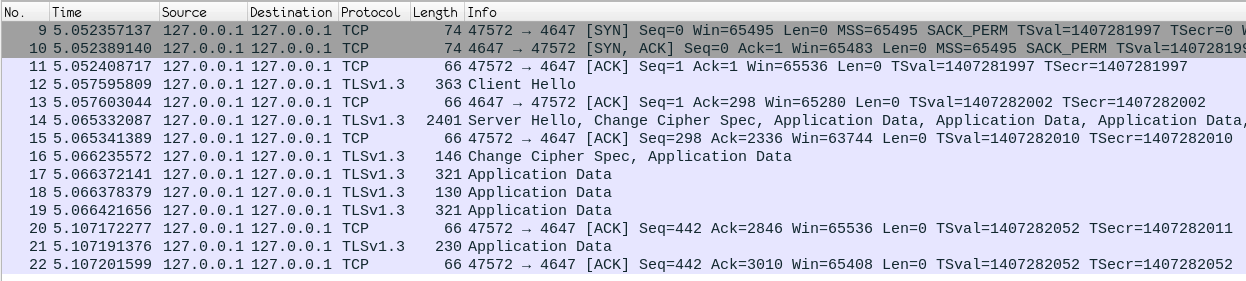
\includegraphics[width=\linewidth]{inc/img/trace-conf-2-tls.png}
  \caption{Сниф wireshark соединения двух участников с использованием TLS}
  \label{img:trace-conf-2-tls}
\end{figure}

\clearpage

На рисунках \ref{img:trace-conf-3}--\ref{img:trace-conf-3-tls} представлены снифы пакетов во время инициализации конференции с тремя участниками. По рисунку видны 3 этапа соединения: инициализация конференции двумя участниками; отправка и получение приглашения для третьего участника и информирование второго участника о новом подключившемся участнике; рукопожатие второго и третьего участников.

\begin{figure}[h!]
  \centering
  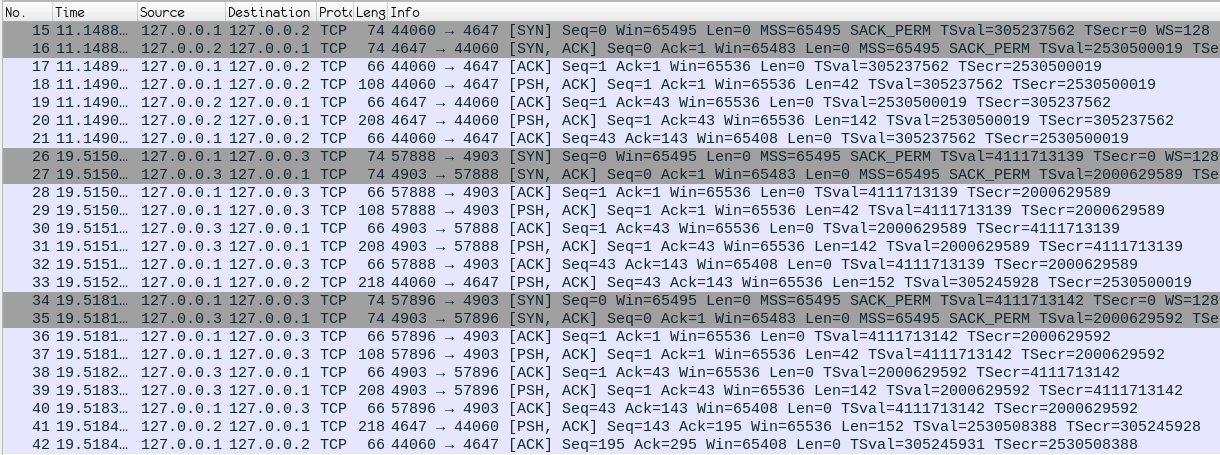
\includegraphics[width=\linewidth]{inc/img/trace-conf-3.png}
  \caption{Сниф wireshark соединения трех участников без использования TLS}
  \label{img:trace-conf-3}
\end{figure}

\begin{figure}[h!]
  \centering
  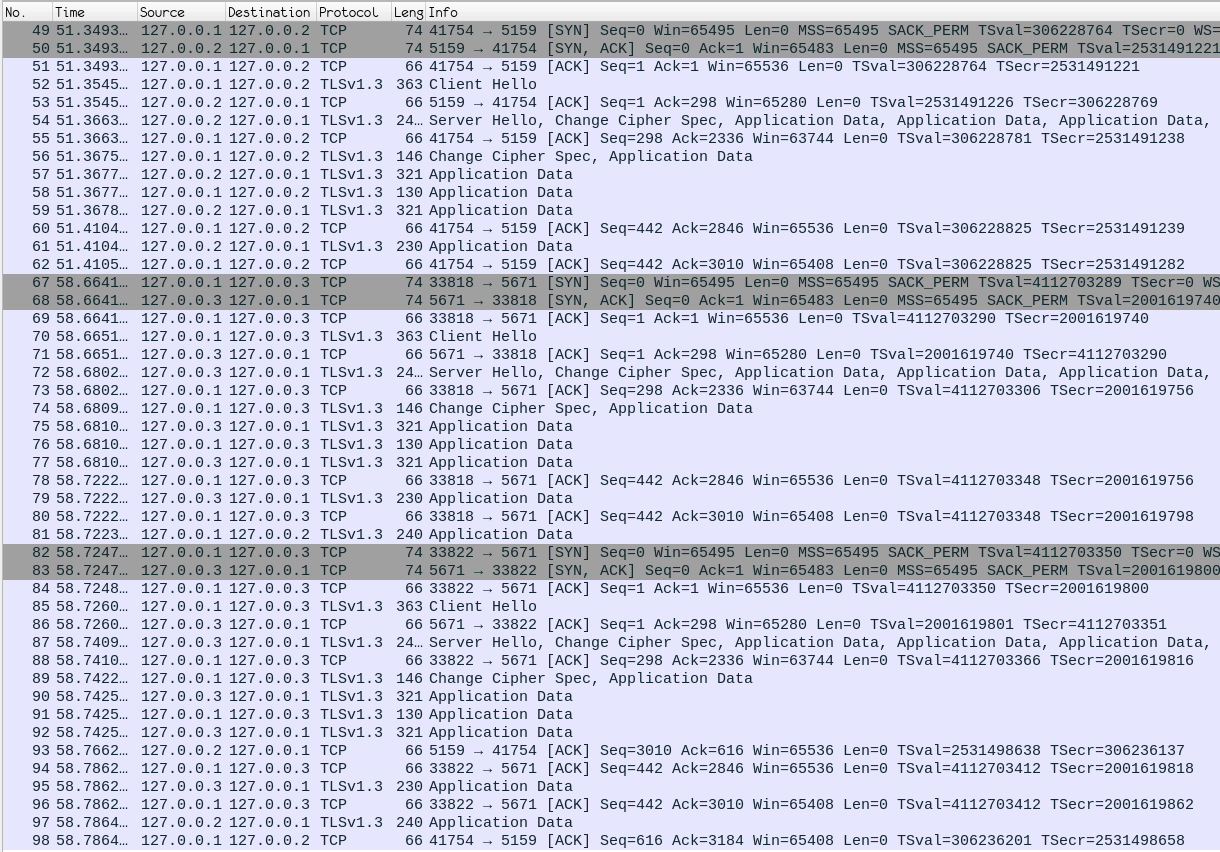
\includegraphics[width=\linewidth]{inc/img/trace-conf-3-tls.png}
  \caption{Сниф wireshark соединения трех участников с использованием TLS}
  \label{img:trace-conf-3-tls}
\end{figure}
